\section{Methods} \label{sec:methods}

This section details the algorithm and implementation design used in this work.
After briefly recounting the core mechanics of hereditary stratigraphy methods for phylogenetic tracking, we motivate and describe new lightweight ``surface'' data structures used to annotate agent genomes in this work.
Then, we describe the asynchronous compute-communicate implementation strategy behind the testbed WSE-oriented island-based genetic algorithm used for validation and benchmarking experiments.

\subsection{Distributed Phylogenetic Tracking}

Natural history of biological life operates under no extrinsic provision for interpretable record-keeping, yet efforts to study it have proved immensely fruitful.
This fact bodes well that scaled-up simulation studies can succeed as a platform for rich hypothesis-driven experiments despite potential sacrifices to aspects of observability currently enjoyed with centralized, storage-rich processing.
Indeed, observational and analytical strategies already developed to confront limitations in biological data can solve, or at least guide, work with massively distributed evolution simulations.

In biology, mutational drift encodes ancestry information in DNA genomes.
Our proposed methods are analogous, with ancestry information captured within genomes themselves rather than external tracking.
Phylogenetic history can then be estimated after the fact, as Figure \ref{fig:runtime-posthoc-schematic} depicts.
This strategy reduces runtime communication and is resilient to germane modes of data loss (e.g., dropped messages, hardware crash-out).

Recent work introducing \textit{hereditary stratigraphy} (hstrat) methodology has explored how best to organize genetic material to maximize reconstruction quality and minimize memory footprint \citep{moreno2022hstrat, moreno2022hereditary}.
Hstrat material can be bundled with agent genomes in a manner akin to non-coding DNA, entirely neutral with respect to agent traits and fitness.

The hereditary stratigraphy algorithm associates each generation along individual lineages with an identifying ``fingerprint'' value, referred to as a differentia.
On birth, offspring receive a new differentia value and append it to an inherited chronological record of past values, each corresponding to a generation along that lineage.
Under this scheme, mismatching differentiae can be used to delimit the extent of common ancestry.
This semantic streamlines \textit{post hoc} phylogenetic reconstruction to a simple trie-building procedure
\citep{moreno2024analysis}.

To save space, differentia may be pruned away.
However, care must be taken to ensure retention of checkpoint generations that maximize coverage across evolutionary history.
Reducing the number of bits per differentia can also provide many-fold memory space savings.
These savings can be re-invested to increase the quantity of differentia retained, improving the density of record coverage across elapsed generations.
The cost of this shift is an increased probability of spurious differentia value collisions, which can make two lineages appear more closely related than they actually are.
We anticipate that most use cases will call for differentia sized on the order of a single bit or a byte.
Indeed, single-bit differentiae have been shown to yield good quality phylogenies using only 96 bits per genome \citep{moreno2024guide}.

Small differentia size intensifies need for a lean data structure to back differentia record management.
Shrinking differentia to a single bit would be absurd if each is accompanied by a 32-bit generational timestamp.
To safely drop timestamps, though, we need means to recalculate them on demand.
As such, all described algorithms include means to deduce timestamps of retained differentia solely from their storage index and the count of the record's elapsed generations.

Lastly, design of hstrat annotations must also consider how available storage space should be allocated across the span of history.
In one possible strategy, retained time points would be distributed evenly across history.
In another, more recent time points would be preferred.
We term these as ``steady'' and ``tilted'' policies, respectively \citep{han2005stream,zhao2005generalized}.
Note that prior hereditary stratigraphy work refers to them instead as ``depth-proportional'' and ``recency-proportional resolution'' \citep{moreno2022hereditary}.
Comparisons of reconstruction quality have shown that tilted policy gives higher quality reconstructions from the same amount of reconstruction space in most --- but not all --- circumstances \citep{moreno2024guide}.
This pattern follows an intuition that high absolute precision is more useful to resolving recent events than more ancient ones.
In practice, it may be desirable to use a hybrid approach that allocates half of available annotation space to each strategy \citep{moreno2024guide}.
The bottom panels of Figure \ref{fig:surf-algorithms} contrast steady versus tilted behaviors.

\subsection{Surface-based Hereditary Stratigraphy Algorithms}

At the outset of this project, several problematic aspects of porting existing hereditary stratigraphy algorithms to the WSE became apparent.
Issues stemmed, in part, from a fundamental feature of these algorithms: organization of retained strata in contiguous, sorted order.
Forthwith, we refer to algorithms following this convention as ``column''-based.
The column design, and attendant implementation details, impose various drawbacks:
\begin{itemize}
\item \textbf{wasted space}: an annotation size cap can be guaranteed, but a percentage of available space typically goes unused;
\item \textbf{high-level feature dependencies:} in places, existing column code uses complex data structures with dynamically allocated memory to perform operations like set subtraction; and
\item \textbf{annotation size scaling:} maintaining sorted order among differentia can take time linearly proportional to annotation size.
\end{itemize}

\begin{figure}[b!]
  \centering
  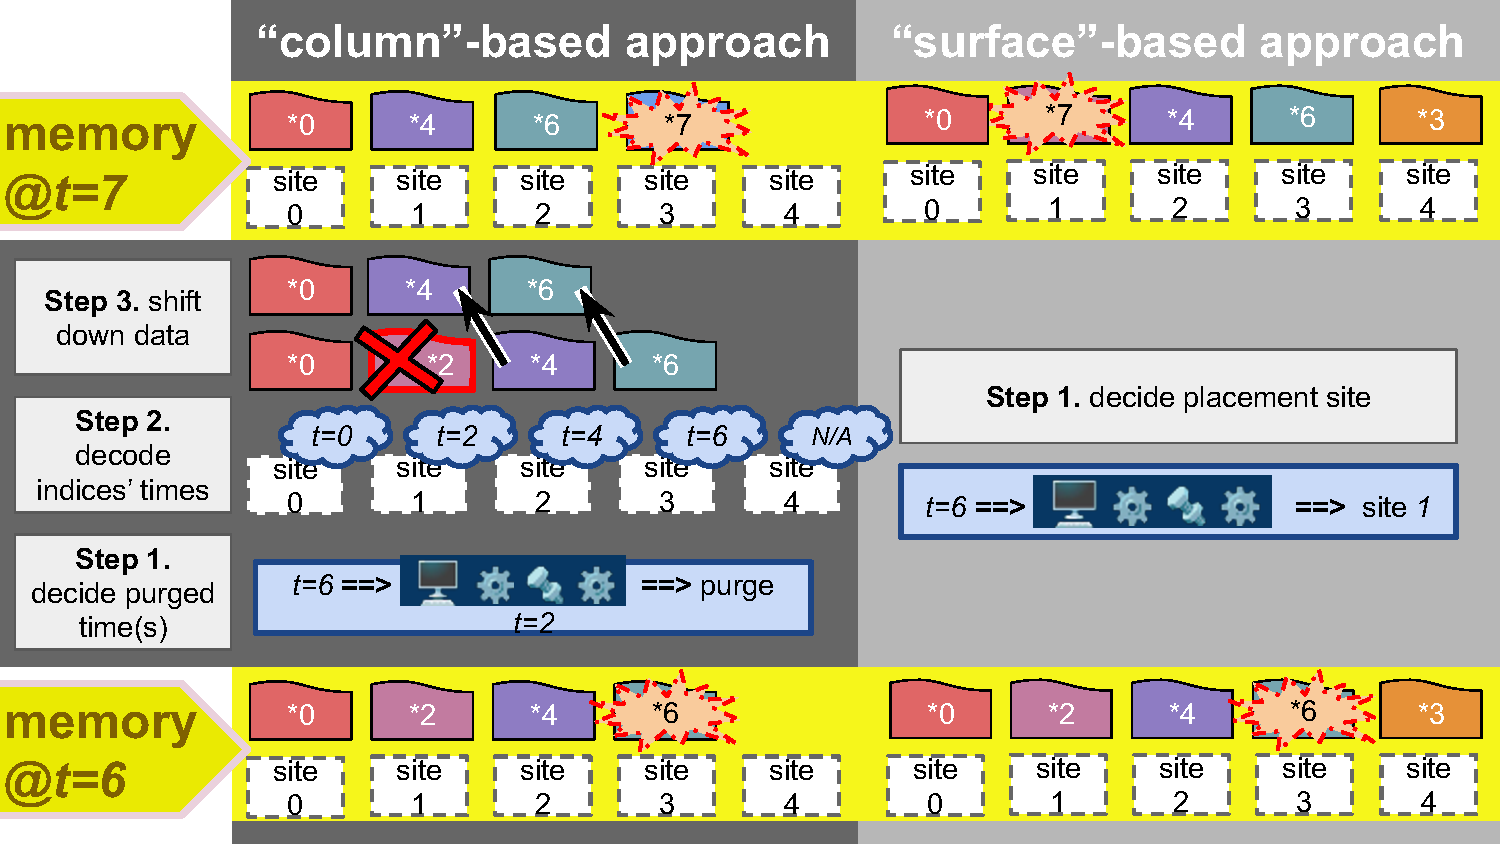
\includegraphics[width=0.95\linewidth]{img/surf-vs-column-schematic}

  \vspace{-1.5ex}

  \caption{
  \textbf{Column vs. surface-based hereditary stratigraphy.}
  \footnotesize
  Contrast of existing sorted-order ``column''-based stratum retention framework with proposed explicitly addressed ``surface''-based approach.}
  \label{fig:surf-vs-column-schematic}
  \vspace{-0.2in}
\end{figure}


\noindent
Addressing these concerns required fundamental reformulation of hereditary stratigraphy conventions.
To this end, we introduce a constant-time indexing scheme that maps each lineage's fingerprint stream directly onto a fixed-width memory buffer.
Differentia pruning occurs implicitly, as a result of resident differentia being overwritten by new placements.
As before, care is taken to guarantee temporally representative collections of resident differentiae within the memory buffer over elapsed time.
We refer to this new approach as ``surface''-based, as opposed to ``column''-based.
Figure \ref{fig:surf-vs-column-schematic} contrasts the two.

\begin{figure*}
  \centering
\begin{subfigure}[b]{0.43\linewidth}
\centering
\textbf{steady retention policy}
\end{subfigure}
\begin{subfigure}[b]{0.43\linewidth}
\centering
\textbf{tilted retention policy}
\end{subfigure}

  \begin{subfigure}[b]{0.43\linewidth}
    \centering
  \includegraphics[height=\linewidth,angle=90,trim={0 2.4cm 0 0},clip]{binder-surface-concept/teeplots/10/cnorm=log+num-generations=4096+surface-size=256+viz=site-deposition-depth-by-rank-heatmap+ynorm=linear+ext=}
    \caption{256 bit steady surface site age plot}
    % \label{fig:runtime-posthoc-schematic}
  \end{subfigure}
  \begin{subfigure}[b]{0.43\linewidth}
    \centering
  \includegraphics[height=\linewidth,angle=90, trim={0 0 0 2.4cm},clip]{binder-surface-concept/teeplots/21/cnorm=log+num-generations=4096+surface-size=256+viz=site-deposition-depth-by-rank-heatmap+ynorm=linear+ext=}
    \caption{256 bit tilted surface site age plot}
    % \label{fig:async-ga-schematic}
  \end{subfigure}


\begin{subfigure}[b]{0.43\linewidth}
  \centering
\includegraphics[width=\linewidth,trim={0 0 0 0},clip]{binder-surface-concept/teeplots/10/num-generations=262144+surface-size=64+viz=stratum-persistence-dripplot+ext=}
  \caption{64 bit steady surface time retention plot}
  % \label{fig:runtime-posthoc-schematic}
\end{subfigure}
\begin{subfigure}[b]{0.43\linewidth}
  \centering
\includegraphics[width=\linewidth,trim={0 0 0 0},clip]{binder-surface-concept/teeplots/21/num-generations=262144+surface-size=64+viz=stratum-persistence-dripplot+ext=}
  \caption{64 bit tilted surface time retention plot}
  % \label{fig:async-ga-schematic}
\end{subfigure}

\caption{%
  Visualizations of steady (left) and tilted (right) surface site selection policies.
  Top row heatmaps shows evolution of time-since-last-deposition for each site on a 256 bit field over the course of 4,096 depositions.
  Bottom row drip plots show retention timelines for 3,000 ingested timepoints.
  Eliminated time points are marked in red.
  Note that for top row, time elapses from top to bottom.
  For bottom row, time elapses bottom to top.
  }
\label{fig:surf-algorithms}

\end{figure*}


In the course of this work, we developed both steady- and tilted-policy surface-based hereditary stratigraphy algorithms.
Figure \ref{fig:surf-algorithms} depicts implementation behaviors, with the top panels tracking how placements are sequenced over time in buffer space and the bottom panels showing the resulting distributions of retained time points across history.
We leave formal descriptions of underlying indexing algorithms to future work.
However, reference Python implementations can be found in provided software materials.
For this work, we also translated the tilted algorithm to the general-purpose Zig programming language and then to the Zig-like Cerebras Software Language for use on the WSE.

These algorithms are notable in providing a novel and highly efficient solution to the more general problem of curating dynamic temporal cross-samples from a data stream, and may lend themselves to a broad set of applications outside the scope of phylogeny tracking \citep{moreno2024algorithms}.

% async microthread to send from sendBuf to neighbor
% fn dispatchSend_S() void {
%   @fmovs(sendDsd_S, sendBufDsd_S,
%     .{
%       .async = true,
%       .activate = sendFinalizeTaskID_S

% const recvDsd_N = @get_dsd(fabin_dsd, .{
%   .fabric_color = recvColor_N,
%   .extent = recvBufSize,
%   .input_queue = @get_input_queue(q_in_N)
% });
% // open an async microthread to recv from neighbor into recvBuf
% fn dispatchRecv_N() void {
%   @fmovs(recvBufDsd_N, recvDsd_N,
%     .{
%       .async = true,

% color swapping

\subsection{WSE Architecture and Programming Model}

The Cerebras Wafer-Scale Engine comprises a networked grid of independently executing compute cores (Processing Elements or PEs).
Each PE contains special message-handling infrastructure, which routes tagged 32-bit packets (``wavelets'') to neighboring PEs and/or to be processed locally, according to a programmed rule set.
Each Processor Element is equipped with 48kb of private on-chip memory, which can be accessed within a single clock cycle;
communication to neighboring PEs, too, incurs low latency \citep{buitrago2021neocortex}.
Processor Elements provide faculties for standard arithmetic and flow-control operations, as well as vectorized 32- and 16-bit integer and floating-point operations.

The WSE device is programmed by providing ``kernel'' code, written in the Cerebras Software Language (CSL), to be executed on each PE.
This language's programming model purposefully reflects underlying capabilities and particularities of the WSE architecture.
CSL organizes code within an event-driven framework, with the programmer defining tasks to be triggered in response to wavelet activation signals exchanged between --- and within --- PEs.
Scheduling of active tasks occurs via hardware-level microthreading, which allows for some level of concurrency.
Special faculties are provided for asynchronous send-receive operations that exchange contiguous, or strided, buffer data between PEs.

For further detail, we refer readers to extensive developer documentation made available by Cerebras through their SDK program.
Access can be requested, currently free of charge, via their website.
For this initial work, we evaluated some CSL code on a virtualized $3\times3$ PE array emulated with conventional CPU hardware, while other experiments used hundreds of thousands of PEs on a physical CS-2 device.

\subsection{Asynchronous Island-model Genetic Algorithm}

\begin{figure}
  \centering
  \begin{subfigure}{0.5\linewidth}
    \centering
    \footnotesize
    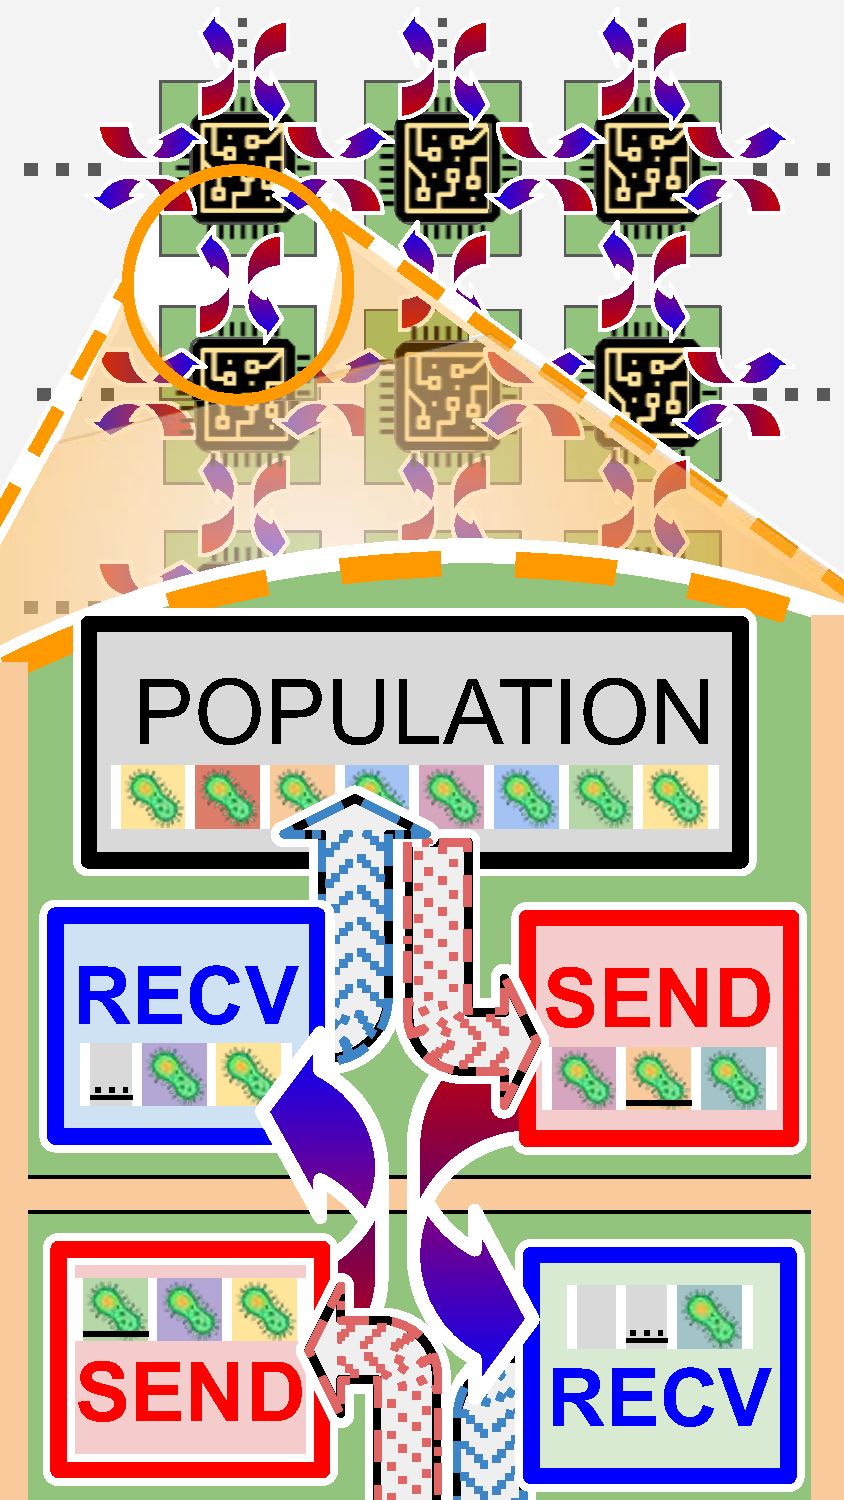
\includegraphics[width=0.8\linewidth]{img/dataflow-schematic}
    \vspace{-0.05in}
    \caption{data flow between PE's}
  \end{subfigure}%
  \begin{subfigure}{0.5\linewidth}
    \footnotesize
    \centering
    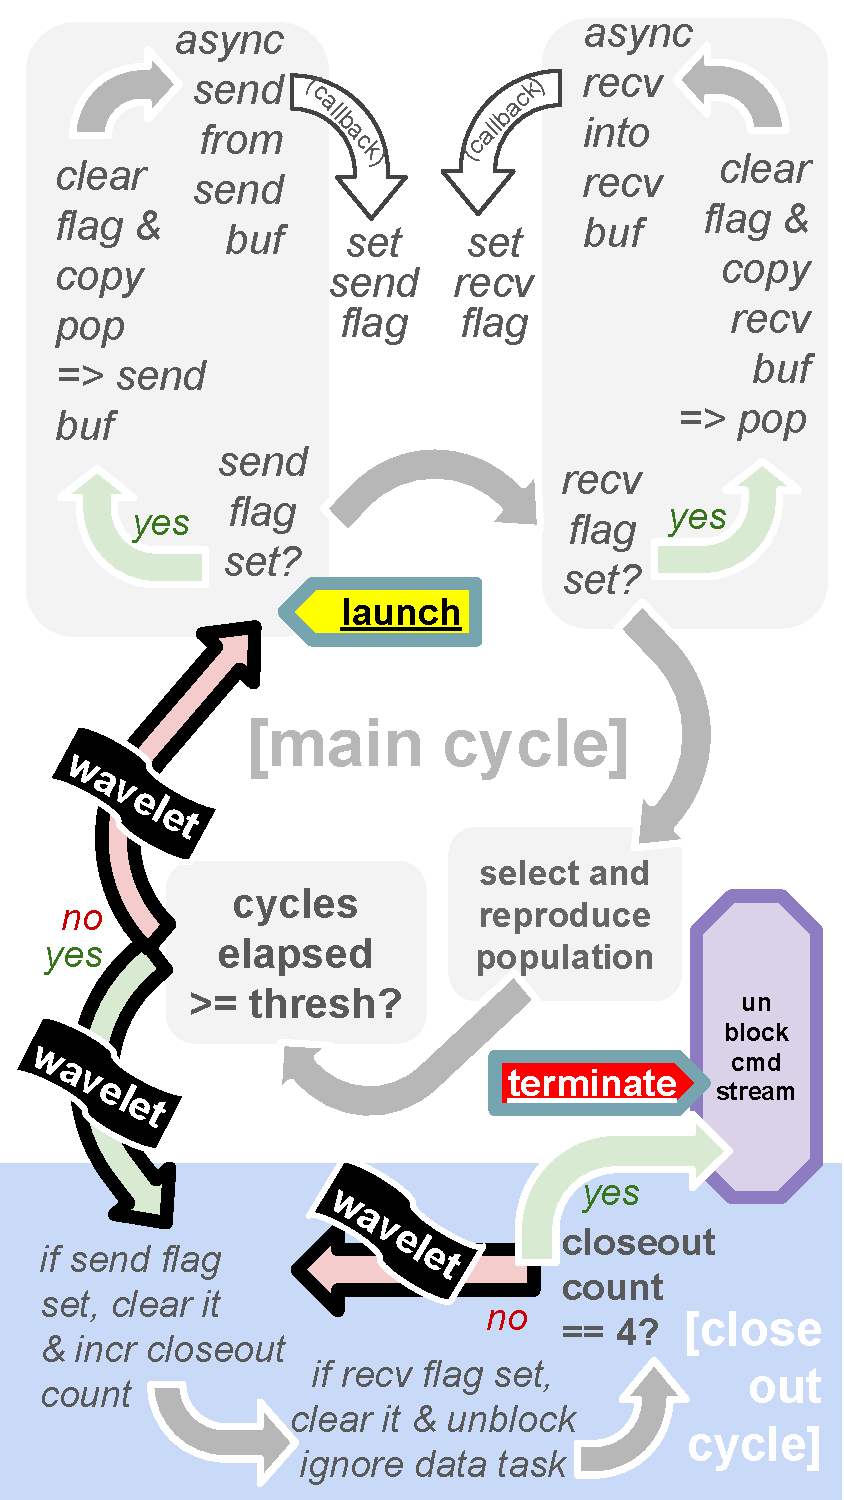
\includegraphics[width=0.8\linewidth]{img/controlflow-schematic}%
    \vspace{-0.05in}
    \caption{control flow within PE}
  \end{subfigure}
  \vspace{-0.25in}
  \caption{%
  \textbf{Island model GA implementation for WSE.}
  \footnotesize
  Neighboring PEs exchange agents (🦠) via asynchronous send/receive operations from dedicated buffers (``migration''), with on-completion callbacks setting ``ready'' flags to copy between main population and ready buffer.
  }
  \label{fig:async-ga-schematic}
  \vspace{-0.2in}
\end{figure}


We apply an island-model genetic algorithm, common in applications of parallel and distributed computing to evolutionary computation, to instantiate a wafer-scale evolutionary process spanning PEs \citep{bennett1999building}.
Under this model, PEs host independent populations that interact through migration (i.e., genome exchange) between neighbors.

Our implementation unfolds according to a generational update cycle, schematized in Figure \ref{fig:async-ga-schematic}.
Migration, depicted as blue-red arrows, is handled first.
Each PE maintains independent immigration buffers and emigration buffers dedicated to each cardinal neighbor, depicted by Figure \ref{fig:async-ga-schematic} in solid blue and red, respectively.
On simulation startup, asynchronous receive operations are opened to accept genomes from each neighboring PE into its corresponding immigration buffer.
At startup, additionally, each emigration buffer is populated with genomes copied from the population and an asynchronous send request is opened for each. %to dispatch wavelets containing genome data from the emigration buffer to the neighbor.
Asynchronous operations are registered to on-completion callbacks that set a per-buffer ``send-'' or ``receive-complete'' flag variable.
In this work, we size send buffers to hold one genome and receive buffers to hold four genomes.
The main population buffer held 32 genomes.

Subsequently, the main update loop tests all completion flags.
For each immigration flag that is set, buffered genomes are copied into the main population buffer, replacing randomly chosen population members.
Then, the flag is reset and a new receive request is initiated.
Likewise, for each emigration flag set, corresponding send buffers are re-populated with randomly sampled genomes from the main population buffer.
Corresponding flags are then reset and new send requests are initiated.
The bottom right corner of Figure \ref{fig:async-ga-schematic} summarizes the interplay between send/receive requests, callbacks, flags and buffers.

The remainder of the main update loop handles evolutionary operations within the scope of the executing PE.
Each genome within the population is evaluated to produce a floating point fitness value.
For this initial work, we use a trivial fitness function that explicitly models additive accumulation of beneficial/deleterious mutations as a floating point value within each genome.
After evaluation, tournament selection is applied.
Each slot in the next generation is populated with the highest-fitness genome among $n=5$ randomly sampled individuals, ties broken randomly.

Finally, a mutational operator is applied across all genomes in the next population.
Experiments used a simple Gaussian mutation on each genome's stored fitness value, with sign restrictions used to manipulate the character of selection in some treatments.
At this point, hereditary stratigraphy annotations --- discussed next --- are updated to reflect an elapsed generation.

The next generation cycle is then launched by a self-activating wavelet, repeating until a generation count halting condition is met.

\subsection{Genome Model}

Genomes were handled as fixed-length segments of raw memory.
We used a 96-bit genome for clade reconstruction trials, shown in Supplementary Figure \ref{fig:genome-layout} \citep{moreno2024supplement}.
At the outset of simulation, the first 16 bits of founding genomes were randomized and, subsequently, were inherited without mutation, thus identifying descendants of the same founding ancestor.
The next 80 bits were used for hereditary stratigraph annotation, 16 bits for a generation counter and the remaining 64 as a field for single-bit differentia managed according to a tilted surface policy.
For other experiments, a 128-bit genome layout was used instead, with the first 32 bits used for a floating point ``fitness'' value and the generation counter upgraded from 16 to 32 bits.
% A key question will be the extent to which intentionally desynchronizing affects performance, stability, and computation quality.

\subsection{Software and Data Availability}

Software, configuration files, and executable notebooks for this work are at \href{https://hopth.ru/cp}{\texttt{hopth.ru/cp}}.
Data and supplemental materials are available via the Open Science Framework at \href{https://hopth.ru/co}{\texttt{hopth.ru/co}} \citep{foster2017open}.

Hereditary stratigraphy utilities are published in the \texttt{hstrat} Python package \citep{moreno2022hstrat}.
This project used data formats from the ALife Standards project \citep{lalejini2019data} and benefited from open-source scientific software \citep{huerta2016ete,2020SciPy-NMeth,harris2020array,reback2020pandas,mckinney-proc-scipy-2010,cock2009biopython,waskom2021seaborn,hunter2007matplotlib,moreno2024apc,moreno2024pecking,moreno2024hsurf,moreno2024wse,dolson2024phylotrackpy}.

WSE experiments reported in this work used the CSL compiler and CS-2 hardware emulator bundled with the Cerebras SDK v1.0.0 \citep{selig2022cerebras}, available via request from Cerebras.
SDK utilities can be run from any Linux desktop environment, regardless of access to Cerebras hardware.
We access hardware through PSC Neocortex \citep{buitrago2021neocortex}.
